%%%%%%%%%%%%%%%%%%%%%%%%%5
%% abtex2-modelo-trabalho-academico.tex, v<VERSION> laurocesar
%% Copyright 2012-<COPYRIGHT_YEAR> by abnTeX2 group at http://www.abntex.net.br/
%%
%% This work may be distributed and/or modified under the
%% conditions of the LaTeX Project Public License, either version 1.3
%% of this license or (at your option) any later version.
%% The latest version of this license is in
%%   http://www.latex-project.org/lppl.txt
%% and version 1.3 or later is part of all distributions of LaTeX
%% version 2005/12/01 or later.
%%
%% This work has the LPPL maintenance status `maintained'.
%%
%% The Current Maintainer of this work is the abnTeX2 team, led
%% by Lauro César Araujo. Further information are available on
%% http://www.abntex.net.br/
%%
%% This work consists of the files abntex2-modelo-trabalho-academico.tex,
%% abntex2-modelo-include-comandos and abntex2-modelo-references.bib
%%

% ------------------------------------------------------------------------
% ------------------------------------------------------------------------
% abnTeX2: Modelo de Trabalho Academico (tese de doutorado, dissertacao de
% mestrado e trabalhos monograficos em geral) em conformidade com
% ABNT NBR 14724:2011: Informacao e documentacao - Trabalhos academicos -
% Apresentacao
% ------------------------------------------------------------------------
% ------------------------------------------------------------------------

\documentclass[
% -- opções da classe memoir --
12pt,				% tamanho da fonte
%  openright,			% capítulos começam em pág ímpar (insere página vazia caso preciso)
oneside,			% para impressão em recto e verso use twoside
a4paper,			% tamanho do papel.
% -- opções da classe abntex2 --
%chapter=TITLE,		% títulos de capítulos convertidos em letras maiúsculas
%section=TITLE,		% títulos de seções convertidos em letras maiúsculas
%subsection=TITLE,	% títulos de subseções convertidos em letras maiúsculas
%subsubsection=TITLE,% títulos de subsubseções convertidos em letras maiúsculas
% -- opções do pacote babel --
english,			% idioma adicional para hifenização
french,				% idioma adicional para hifenização
spanish,			% idioma adicional para hifenização
brazil				% o último idioma é o principal do documento
]{abntex2}

% ---
% Pacotes básicos
% ---
\usepackage{times}			    % Usa fonte times
\renewcommand{\ABNTEXchapterfont}{\normalfont} % para aplicar a fonte escolhida em tudo
\usepackage[T1]{fontenc}		% Selecao de codigos de fonte.
\usepackage[utf8]{inputenc}		% Codificacao do documento (conversão automática dos acentos)
\usepackage{lastpage}			% Usado pela Ficha catalográfica
\usepackage{indentfirst}		% Indenta o primeiro parágrafo de cada seção.
\usepackage{color}				% Controle das cores
\usepackage{graphicx}			% Inclusão de gráficos
\usepackage{microtype} 			% para melhorias de justificação
\usepackage{parselines} 
% ---

% ---
% Pacotes adicionais, usados apenas no âmbito do Modelo Canônico do abnteX2
% ---
\usepackage{lipsum}				% para geração de dummy text
% ---

% ---
% Pacotes de citações
% ---
\usepackage[brazilian,hyperpageref]{backref}	 % Paginas com as citações na bibl
\usepackage[$referencias_sistema$]{abntex2cite}	% Citações padrão ABNT

% ---
% CONFIGURAÇÕES DE PACOTES
% ---

% ---
% Configurações do pacote backref
% Usado sem a opção hyperpageref de backref
\renewcommand{\backrefpagesname}{Citado na(s) página(s):~}
% Texto padrão antes do número das páginas
\renewcommand{\backref}{}
% Define os textos da citação
\renewcommand*{\backrefalt}[4]{
	\ifcase #1 %
	Nenhuma citação no texto.%
	\or
	Citado na página #2.%
	\else
	Citado #1 vezes nas páginas #2.%
	\fi}%
% ---

% ---
% Informações de dados para CAPA e FOLHA DE ROSTO
% ---


\titulo{Teste}
\autor{João Fernando\\Felipe Augusto}

\data{2025}
\local{São Paulo - SP}
%\orientador{$orientador$}
%\coorientador{$coorientador$}
\instituicao{UNIVERSIDADE VIRTUAL DO ESTADO DE SÃO PAULO\\}
\tipotrabalho{Vídeo de apresentação do Projeto Integrador: \\
<https://youtu.be/odasdasdas>}


% O preambulo deve conter o tipo do trabalho, o objetivo (propósito),
% o nome da instituição e a área de concentração.
% Esse texto irá compor a Folha de Rosto e Folha de Aprovação.
\preambulo{ Relatório Técnico-Científico apresentado na	disciplina de Projeto Integrador para o curso de Licenciatura em Matemática da Universidade	Virtual do Estado de São Paulo (UNIVESP).}
% fim do preambulo
% ---


% Configurações de aparência do PDF final

% alterando o aspecto da cor azul
\definecolor{blue}{RGB}{41,5,195}

% informações do PDF
\makeatletter
\hypersetup{
	%pagebackref=true,
	pdftitle={\@title},
	pdfauthor={\@author},
	pdfsubject={\imprimirpreambulo},
	pdfcreator={LaTeX with abnTeX2 and Limarka},
	pdfkeywords={abnt}{latex}{abntex}{abntex2}{trabalho acadêmico}{limarka},
	colorlinks=false,       		% false: boxed links; true: colored links
	linkcolor=black,          	% color of internal links
	citecolor=black,        		% color of links to bibliography
	filecolor=black,      		% color of file links
	urlcolor=black,
	bookmarksdepth=4
}
\makeatother
% ---

% ---
% Possibilita criação de Quadros e Lista de quadros.
% Ver https://github.com/abntex/abntex2/issues/176
%
\newcommand{\quadroname}{Quadro}
\newcommand{\listofquadrosname}{Lista de quadros}

\newfloat[chapter]{quadro}{loq}{\quadroname}
\newlistof{listofquadros}{loq}{\listofquadrosname}
\newlistentry{quadro}{loq}{0}

% configurações para atender às regras da ABNT
\setfloatadjustment{quadro}{\centering}
\counterwithout{quadro}{chapter}
\renewcommand{\cftquadroname}{\quadroname\space}
\renewcommand*{\cftquadroaftersnum}{\hfill--\hfill}

% ---

% --- GERAR CAPA
\renewcommand{\imprimircapa}{%
	\begin{capa}%
		
		\center
		\ABNTEXchapterfont\Large \imprimirinstituicao
		\vspace*{2cm}
		{\setlength{\parskip}{0.01cm}\ABNTEXchapterfont\large\imprimirautor}
		\vfill
		\begin{center}
			\ABNTEXchapterfont\bfseries\LARGE\imprimirtitulo
		\end{center}
		\begin{center}
			\imprimirtipotrabalho			
		\end{center}
		\vfill
		\large\imprimirlocal\\
		\large\imprimirdata
		\vspace*{1cm}

	\end{capa}
}


% --- GERAR FOLHA DE ROSTO

\makeatletter
\renewcommand{\folhaderostocontent}{


\begin{center}
	{\ABNTEXchapterfont\large\imprimirautor}
	\vspace*{\fill}\vspace*{\fill}
	\begin{center}
		\ABNTEXchapterfont\bfseries\Large\imprimirtitulo
	\end{center}
	\vspace*{\fill}
	\abntex@ifnotempty{\imprimirpreambulo}{%
		\hspace{.45\textwidth}
		\begin{minipage}{.48\textwidth}
			\SingleSpacing
			\imprimirpreambulo
		\end{minipage}%
		\vspace*{\fill}
	}%
%	{\abntex@ifnotempty{\imprimirinstituicao}{\imprimirinstituicao
%			\vspace*{\fill}}}
	{\large\imprimirorientadorRotulo~\imprimirorientador\par}
	\abntex@ifnotempty{\imprimircoorientador}{%
		{\large\imprimircoorientadorRotulo~\imprimircoorientador}%
	}%
	\vspace*{\fill}
	{\large\imprimirlocal}
	\par
	{\large\imprimirdata}
	\vspace*{1cm}
\end{center}
}
\makeatother


% ---
% Espaçamentos entre linhas e parágrafos
% ---

% O tamanho do parágrafo é dado por:
\setlength{\parindent}{1.3cm}

% Controle do espaçamento entre um parágrafo e outro:
\setlength{\parskip}{0.2cm}  % tente também \onelineskip

% ---
% compila o indice
% ---
\makeindex
% ---

%---
% CONFIGURAÇÕES EXTRA DO LIMARKA
%---

% Configura citações de pandoc para 4cm à esquerda (utiliza o ambiente quote)
\renewenvironment{quote}
{\small\list{}{\rightmargin=0.1cm \leftmargin=4cm}%
	\item\relax}
{\endlist}

% Para incluir páginas PDF (ficha catalografica e folha de aprovação)
\usepackage[dvipsnames]{xcolor} % http://tex.stackexchange.com/questions/124636/package-xcolor-error-undefined-colors-maroon-royal-blue-when-master-has-pdf
\usepackage{pdfpages}
\usepackage{longtable,ltcaption,booktabs} % para as tabelas pandoc e quadros ABNT
%\usepackage{floatrow}
%\floatsetup[figure]{capposition=top}

% Para melhorar o visual do quadro
\usepackage{boldline} 
\def\toprule{\hlineB{3}} % primeira linha mais gorda
\def\midrule{\hline}
\def\bottomrule{\hlineB{3}} % última linha mais gorda



% ---
% BUG: Imagens e tabelas apareciam no meio da página em branco
% https://github.com/abntex/trabalho-academico-limarka/issues/1
% O código a seguir posta imagens ou tabelas em página em branco no topo, em vez do meio (comportamento padrão)
\makeatletter
\setlength{\@fptop}{5pt} % Set distance from top of page to first float
\makeatother
% ---

% ---
% Usado pelo limarka como hook para criação de novas listas.
% https://github.com/abntex/trabalho-academico-limarka/issues/16
%
\newcommand{\listasdousuario}{}

% ---
% CUSTOMIZAÇÕES DO USUÁRIO (somente se existir arquivo latexcustomizacao.sty)
% ---
\IfFileExists{latexcustomizacao.sty}{\usepackage{latexcustomizacao}}{}

%%
%% Esse modelo é responsável pela impressão dos seguintes elementos:
%% Capa, Folha de rosto e Ficha catalográfica.

\special{dvipdfmx:config z 0}

% ----
% Início do documento
% ----
\begin{document}
	
	% Seleciona o idioma do documento (conforme pacotes do babel)
	%\selectlanguage{english}
	\selectlanguage{brazil}
	
	% Retira espaço extra obsoleto entre as frases.
	\frenchspacing
	
	% ----------------------------------------------------------
	% ELEMENTOS PRÉ-TEXTUAIS
	% ----------------------------------------------------------
	% \pretextual
	
	
	% Gerando capa abnTeX2
	\imprimircapa
	% ---
	
	% ----------------------------------------------------------
	% ELEMENTOS PRÉ-TEXTUAIS
	% ----------------------------------------------------------
	% \pretextual
	
	\imprimirfolhaderosto*
	
	% EDIÇÃO E INCLUSÃO DOS ELEMENTOS PRÉ-TEXTUAIS

%-------------------------------------------
% Inserir resumo
%-------------------------------------------
\setlength{\absparsep}{18pt} % ajustando espaçamento dos paragrafos do resumo
\begin{resumo}
	Segundo .....
	
	\textbf{PALAVRAS-CHAVE}: matemática, univesp...
\end{resumo}

%-------------------------------------------
% Inserir lista de ilustrações
%-------------------------------------------

\pdfbookmark[0]{\listfigurename}{lof}
\listoffigures*
\clearpage

%-------------------------------------------
% Inserir sumário
%-------------------------------------------

\pdfbookmark[0]{\contentsname}{toc}
\tableofcontents*
\clearpage

% FINAL DOS ELEMENTOS PRÉ TEXTUAIS
	
	% ----------------------------------------------------------
	% ELEMENTOS TEXTUAIS
	% ----------------------------------------------------------
	\textual
	\pagestyle{simple}                  % #17 Cabeçalho apenas com
	\aliaspagestyle{chapter}{simple}    % a numeração das páginas
	
	
	\pagestyle{simple}
\chapter[]{Introdução}
A violência representa uma ameaça ao processo educacional ensino aprendizagem, e isso pode ocasionar consequências a curto e a longo prazo na vida de uma pessoa. A palavra bullying pode ser bem definido como um ato de praticar ou se envolver em violência, seja ela física ou psicológica, de comportamento agressivo intencional e negativo com execução repetida da ação, envolvendo crianças que apresentam relacionamento com desequilíbrio de poder. Em muitos casos o bullying ocorre como forma de apelido, ofensas, agressão, bater, intimidar, zoar. Sendo estas, formas diretas ou indiretas da praticas do bullying. 

No Brasil, adotou-se o termo bullying, que é utilizado na maioria dos países. Sua definição é compreendida como um subconjunto de comportamentos agressivos, sendo de natureza repetitiva e caracterizada por um desequilíbrio de poder. \citeonline{CleoFante} comenta que para alguns pesquisadores são necessários no mínimo três ataques contra a vítima no decorrer do ano para ser configurado como bullying. Na mesma direção o pesquisador \citeonline{DanOlweus}, afirma que o bullying ocorre quando ações violentas são reproduzidas de três a cinco vezes ao ano. 

A agressividade pode estar ligada a diversos fatores, exemplos: transtorno, distúrbio, influência de amigos e familiares, ou seja a violência na escola está ligada ao contexto social, familiar e escolar. \citeonline{BeatrizPereira} descreve o bullying como uma forma de comportamento agressivo, geralmente maldosa, deliberada e com frequência persistente, podendo durar semanas, meses ou anos, sendo as vítimas sempre incapazes de se defender. O autor ainda acrescenta que, três características são básicas para diferenciar o bullying de outros tipos de violência: o mal causado não resulta de provocações; as intimidações são regulares, os agressores em geral são mais fortes e violentos e as vítimas não estão preparadas para se defender. 

Dentro da proposta temática do multiculturalismo, optamos por abordar especificamente o tema do bullying físico. O projeto foi desenvolvido com os alunos do 3º ano do Ensino Fundamental da Escola Estadual Presidente João Goulart (Figura \ref{fig:fachada_escola}), localizada no extremo sul de São Paulo/SP. 

Como recurso pedagógico, utilizamos a literatura infantil, trabalhando com o livro "E se fosse você?", da escritora Sandra Saruê. A obra serviu como ponto de partida para reflexões e atividades sobre empatia, respeito às diferenças e as consequências do bullying no ambiente escolar. 

\begin{figure}
	\centering
	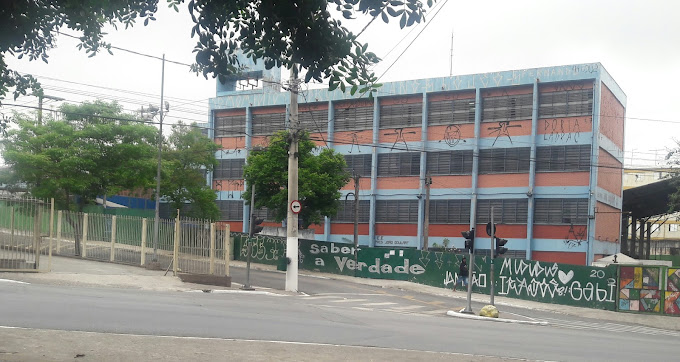
\includegraphics[width=0.75\textwidth]{fachada1.jpg}
	\caption{Fachada da E. E. Prof João Goulart}
	\label{fig:fachada_escola}
\end{figure}

\chapter{Desenvolvimento}
O desenvolvimento deste projeto foi pautado em uma pesquisa de campo, com a realização de um estudo de caso junto aos alunos do 3º ano do Ensino Fundamental da Escola Estadual Presidente João Goulart, situada no extremo sul da cidade de São Paulo/SP. 

A partir da observação direta e da interação com a comunidade escolar e o entorno, foram identificadas situações recorrentes de desrespeito entre os alunos, como o uso de apelidos ofensivos, agressões físicas e verbais, exclusão social e comportamentos indisciplinados. Essas evidências revelam um cenário preocupante, que compromete tanto o ambiente escolar quanto o processo de ensino aprendizagem. 

Diante desse contexto, a equipe de pesquisa propôs o desenvolvimento do projeto “Promovendo o respeito às diferenças e combatendo o bullying na escola”, com o objetivo de fomentar uma cultura de paz, por meio de leituras significativas, atividades reflexivas e diálogos sobre a valorização da diversidade e a construção de uma ética multicultural. 

Com isso, nosso grupo acredita que a proposta pedagógica busca não apenas intervir nas relações interpessoais dos alunos, mas também estimular uma reflexão coletiva sobre as práticas escolares e os desafios da convivência em contextos marcados por desigualdades sociais, preconceitos e discriminações. 

\section{OBJETIVOS}
\textbf{Objetivo Geral}\\
O principal objetivo do projeto será promover a conscientização dos alunos sobre o bullying físico, suas causas e consequências, incentivando atitudes de respeito, empatia e valorização das diferenças no ambiente escolar. 

\textbf{Objetivo Específico}\\
Estimular o diálogo entre os alunos sobre experiências pessoais e coletivas relacionadas ao tema;

Desenvolver a capacidade de se colocar no lugar do outro por meio da leitura e interpretação da obra literária;

Trabalhar valores ligados ao multiculturalismo, como tolerância, inclusão e convivência pacífica;

Utilizar a literatura como ferramenta pedagógica para abordar questões sociais e emocionais relevantes para a faixa etária.

\section{JUSTIFICATIVA E DELIMITAÇÃO DO PROBLEMA}

Esse projeto justifica-se pela necessidade urgente de enfrentar práticas de bullying físico no ambiente escolar, especialmente em instituições públicas localizadas em regiões mais periféricas, onde as vulnerabilidades sociais são mais visíveis, como é o caso da E.E. Pres. João Goulart, situada no extremo sul da cidade de São Paulo. A ideia é abordar o assunto com os estudantes desenvolvendo habilidades socioemocionais para combater essa prática.

A observação direta realizada com os alunos do 3º ano do ensino fundamental evidenciou comportamentos preocupantes como apelidos ofensivos, agressões físicas, exclusão social e atitudes de desrespeito entre os estudantes. Essas condutas afetam diretamente o ambiente escolar, prejudicando não apenas o rendimento acadêmico, mas também o bem-estar social e emocional dos alunos envolvidos.

Diante desse cenário, a escola vê desafiada a ir além do currículo tradicional, adotando uma abordagem mais humanizada, voltada a formação ética e cidadã. Acreditamos que a escola, enquanto espaço de convivência e construção coletiva, pode e deve promover valores como o respeito, empatia, tolerância e inclusão, especialmente por meio de metodologias que favoreçam o diálogo e a escuta ativa.

A utilização da literatura infantil, representada aqui pelo livro “E Se Fosse Com Você, Uma História de Bullying”, da Sandra Saruê, possibilita trabalhar tais valores de forma sensível, acessível e significativa para alunos nessa faixa etária. 


\section{FUNDAMENTAÇÃO TEÓRICA}

A escola é um espaço essencial de formação integral, onde crianças desenvolvem não apenas competências cognitivas, mas também valores, atitudes e habilidades sociais fundamentais para a convivência em sociedade. No entanto, esse ambiente nem sempre é isento de conflitos, sendo o bullying um dos fenômenos mais recorrentes e prejudiciais ao processo de ensino aprendizagem e à saúde emocional dos alunos.

\textbf{Bullying físico no contexto escolar}

O bullying pode ser definido como um comportamento agressivo, intencional e repetitivo, que ocorre dentro de uma relação de desequilíbrio de poder entre as partes envolvidas \citeonline{DanOlweus}. No caso do bullying físico, essas agressões manifestam-se por meio de empurrões, socos, tapas, chutes e outras formas de violência corporal, frequentemente acompanhadas por ofensas verbais e exclusão social.

\begin{citacao}
	Segundo Menezes, o bullying físico é um dos tipos mais visíveis e, ao mesmo tempo, um dos mais ignorados quando naturalizado no cotidiano escolar como "brincadeiras" ou "coisas de criança". No entanto, suas consequências são graves: afetam o rendimento escolar, a autoestima, a saúde mental das vítimas e, muitas vezes, perpetuam um ciclo de violência. \cite[p.123-138]{IzabelMenezes} 
\end{citacao}


\textbf{Educação multicultural e respeito às diferenças}

Para enfrentar esse tipo de violência, é essencial que a escola adote uma abordagem que valorize a diversidade e promova o respeito às diferenças culturais, étnicas, sociais, religiosas e físicas. A educação multicultural tem como objetivo principal construir um ambiente escolar que reconheça e respeite as identidades diversas dos alunos, desconstruindo preconceitos e práticas excludentes.

Segundo \cite{Candau}, a educação multicultural é um caminho para a construção de uma sociedade mais justa, pois permite que as crianças aprendam desde cedo a conviver com o outro de forma ética e solidária. Nesse sentido, combater o bullying também passa por cultivar a empatia, o diálogo e a consciência crítica sobre os efeitos da desigualdade e da intolerância nas relações escolares.

\textbf{A literatura infantil como recurso pedagógico}

A literatura infantil se apresenta como uma ferramenta potente para mediar reflexões sobre temas complexos como o bullying e o respeito à diversidade. Conforme afirma \cite{Coelho}, a literatura tem a capacidade de ampliar o universo simbólico das crianças, despertando sentimentos, promovendo a identificação com personagens e estimulando a reflexão sobre valores humanos.

No caso deste projeto, o livro "E se fosse você?", de Sandra Saruê, foi escolhido por abordar, de maneira sensível e acessível, situações de exclusão, preconceito e bullying, incentivando o leitor a se colocar no lugar do outro. Essa estratégia pedagógica permite trabalhar conceitos como empatia, solidariedade e respeito de forma significativa, adaptada à faixa etária dos alunos envolvidos. 

\textbf{A pedagogia do diálogo e da escuta}

Com base na pedagogia crítica de Paulo \citeonline{PauloFreire}, é fundamental que a educação seja construída a partir do diálogo, da escuta e do respeito às experiências dos alunos. O combate ao bullying não se faz com punições isoladas, mas com processos educativos que envolvam toda a comunidade escolar na construção de uma cultura de paz, justiça e responsabilidade coletiva.

\section{METODOLOGIA}

O presente projeto será desenvolvido com a turma do 3º ano do Ensino Fundamental da E.E. Pres. João Goulart, situada no extremo sul de São Paulo/SP, durante o ano letivo vigente.

A metodologia adotada será de caráter qualitativo, baseada em um estudo de caso, que prevê a observação, a interação e a intervenção pedagógica junto aos alunos. As etapas principais serão:

\textbf{Diagnóstico inicial}

Realização de observações em sala de aula e nos momentos de convivência escolar para identificar comportamentos relacionados ao bullying físico e suas possíveis causas, além de entrevistas e conversas informais com professores e alunos para compreender a dinâmica do grupo.

\textbf{Uso da literatura infantil como recurso pedagógico}

Introdução do livro “E se fosse você?”, de Sandra Saruê, para a leitura compartilhada em roda de conversa. A obra será utilizada para estimular a empatia, a reflexão e o diálogo sobre as consequências do bullying e a importância do respeito às diferenças


\textbf{Atividades lúdicas e reflexivas}

Proposição de atividades como dramatizações, debates, produções artísticas (desenhos, cartazes, textos) e dinâmicas de grupo, com o objetivo de reforçar os conceitos discutidos durante as rodas de conversa e ampliar a compreensão sobre convivência pacífica.

\textbf{Envolvimento da comunidade escolar}

Organização de encontros com professores, e equipe pedagógica para compartilhar os objetivos do projeto, discutir estratégias de prevenção ao bullying e fortalecer uma rede de apoio à promoção do respeito no ambiente escolar.

\textbf{Registro e análise dos processos}

Documentação das atividades, observações e relatos para acompanhar o desenvolvimento dos alunos e o impacto das ações, possibilitando ajustes na metodologia conforme as necessidades identificadas.


\section{RESULTADOS PRELIMINARES: SOLUÇÃO INICIAL}

Diante do diagnóstico realizado junto aos alunos do 3º ano do Ensino Fundamental da Escola Estadual Presidente João Goulart, que evidenciou a presença de comportamentos de bullying físico, o projeto propõe como solução inicial a utilização do livro “E se fosse você?”, de Sandra Saruê, como recurso pedagógico central.

A estratégia consiste em promover rodas de conversa, leituras compartilhadas e atividades lúdicas que incentivem a empatia e o respeito às diferenças, favorecendo a reflexão sobre as consequências das atitudes agressivas e a valorização da diversidade.

Espera-se que, por meio dessas atividades, os alunos desenvolvam maior consciência sobre o impacto do bullying, reconheçam o valor da convivência pacífica e aprimorem suas habilidades sociais para resolver conflitos de maneira não violenta.

Embora ainda não tenha sido implantado, acredita-se que essa abordagem pedagógica, centrada na literatura infantil e no diálogo, será eficaz para reduzir as práticas de bullying físico e promover um ambiente escolar mais acolhedor e seguro.


%\chapter{Resultados}

%\begin{figure}
%	\centering
%	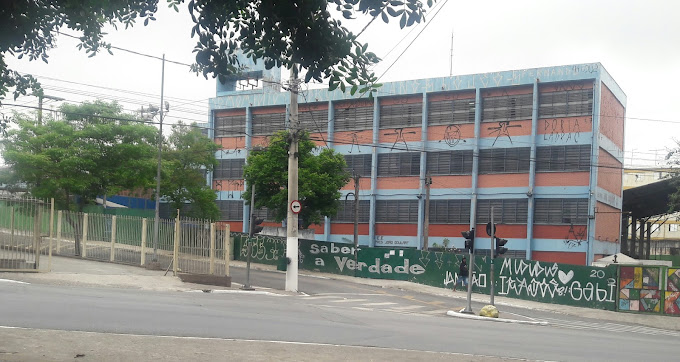
\includegraphics[width=0.65\textwidth]{fachada1.jpg}
%	\caption{Fachada da E. E. Prof João Goulart}
%	\label{fig:fachada_escola2}
%\end{figure}

%\chapter{Considerações Finais}
%
%\lipsum[1-5]	


	% ----------------------------------------------------------
	% ELEMENTOS PÓS-TEXTUAIS
	% ----------------------------------------------------------
	\postextual
	% ----------------------------------------------------------
	
\chapter{POS TEXTUAIS}
	
\end{document}